%%%%%%%%%%%%%%%%%%%%%%%%%%%%%%%%%%%%%%%%%%%%%%%%%%%%%%%%%%%%%%%%%%%%%%%%%%%%%%%
%% RAPPORT DE PROJET HPC - GOLOMB RULER SOLVER
%% Master 1 - Calcul Haute Performance / Imagerie / IA
%% Université de Reims Champagne-Ardenne
%%%%%%%%%%%%%%%%%%%%%%%%%%%%%%%%%%%%%%%%%%%%%%%%%%%%%%%%%%%%%%%%%%%%%%%%%%%%%%%

\documentclass[12pt,a4paper,twoside]{report}

%% ============================================================================
%% PACKAGES
%% ============================================================================

% Encodage et langue
\usepackage[utf8]{inputenc}
\usepackage[T1]{fontenc}
\usepackage[french,provide=*]{babel}

% Mise en page
\usepackage[top=2.5cm, bottom=2.5cm, left=2.5cm, right=2.5cm]{geometry}
\linespread{1.3}

% Mathématiques
\usepackage{amsmath,amssymb,amsthm}
\usepackage{mathtools}

% Graphiques et schémas
\usepackage{tikz}
\usetikzlibrary{shapes,arrows,positioning,calc,fit,backgrounds,decorations.pathreplacing,matrix,3d}
\usepackage{pgfplots}
\pgfplotsset{compat=1.18}
\usepackage{graphicx}
\graphicspath{{images/}}

% Tableaux
\usepackage{booktabs}
\usepackage{tabularx}
\usepackage{multirow}
\usepackage{array}

% Code et algorithmes
\usepackage{listings}
\usepackage[ruled,vlined,french,linesnumbered]{algorithm2e}
\SetAlgorithmName{Algorithme}{algorithme}{Liste des algorithmes}

% Boîtes colorées
\usepackage{tcolorbox}
\tcbuselibrary{theorems,skins,breakable}

% Références et liens
\usepackage{hyperref}
\hypersetup{
    colorlinks=true,
    linkcolor=blue!60!black,
    citecolor=green!50!black,
    urlcolor=blue!70!black
}
\usepackage{cleveref}

% Divers
\usepackage{xcolor}
\usepackage{subcaption}
\usepackage{siunitx}
\usepackage{fancyhdr}
\usepackage{enumitem}

%% ============================================================================
%% CONFIGURATION DES LISTINGS
%% ============================================================================

\definecolor{codegreen}{rgb}{0,0.6,0}
\definecolor{codegray}{rgb}{0.5,0.5,0.5}
\definecolor{codepurple}{rgb}{0.58,0,0.82}
\definecolor{backcolour}{rgb}{0.97,0.97,0.97}

\lstdefinestyle{cppstyle}{
    language=C++,
    backgroundcolor=\color{backcolour},
    commentstyle=\color{codegreen},
    keywordstyle=\color{blue}\bfseries,
    numberstyle=\tiny\color{codegray},
    stringstyle=\color{codepurple},
    basicstyle=\ttfamily\small,
    breakatwhitespace=false,
    breaklines=true,
    captionpos=b,
    keepspaces=true,
    numbers=left,
    numbersep=5pt,
    showspaces=false,
    showstringspaces=false,
    showtabs=false,
    tabsize=4,
    frame=single,
    framerule=0.5pt,
    morekeywords={alignas,atomic,uint64_t,__m256i}
}
\lstset{style=cppstyle}

%% ============================================================================
%% ENVIRONNEMENTS PERSONNALISÉS
%% ============================================================================

\newtcbtheorem[number within=chapter]{definition}{Définition}{
    colback=blue!5,
    colframe=blue!50!black,
    fonttitle=\bfseries,
    breakable
}{def}

\newtcbtheorem[number within=chapter]{theoreme}{Théorème}{
    colback=green!5,
    colframe=green!50!black,
    fonttitle=\bfseries,
    breakable
}{thm}

\newtcbtheorem[number within=chapter]{probleme}{Problème Rencontré}{
    colback=red!5,
    colframe=red!60!black,
    fonttitle=\bfseries,
    breakable
}{prob}

\newtcbtheorem[number within=chapter]{solution}{Solution Implémentée}{
    colback=green!5,
    colframe=green!60!black,
    fonttitle=\bfseries,
    breakable
}{sol}

%% ============================================================================
%% EN-TÊTES ET PIEDS DE PAGE
%% ============================================================================

\pagestyle{fancy}
\fancyhf{}
\fancyhead[LE,RO]{\thepage}
\fancyhead[RE]{\leftmark}
\fancyhead[LO]{\rightmark}
\renewcommand{\headrulewidth}{0.4pt}

%% ============================================================================
%% INFORMATIONS DU DOCUMENT
%% ============================================================================

\title{
    \vspace{-2cm}
    \includegraphics[width=0.3\textwidth]{logo_urca.png}\\[1cm]
    {\Huge\bfseries Solveur de Règles de Golomb\\[0.3cm]
    \Large Optimisation et Parallélisation sur Cluster HPC}\\[1cm]
    \large Rapport de Projet --- Master 1 HPC/Imagerie/IA
}

\author{
    \textbf{Étudiant :} Nicolas\\[0.5cm]
    \textbf{Encadrant :} [Nom de l'encadrant]\\[0.5cm]
    \textbf{Institution :} Université de Reims Champagne-Ardenne\\
    CReSTIC --- Centre de Recherche en STIC
}

\date{Année universitaire 2024--2025}

%% ============================================================================
%% DÉBUT DU DOCUMENT
%% ============================================================================

\begin{document}

% Page de titre personnalisée (sans logo si non disponible)
\begin{titlepage}
    \centering
    \vspace*{1cm}

    {\scshape\LARGE Université de Reims Champagne-Ardenne\par}
    \vspace{0.5cm}
    {\scshape\large Master 1 --- Calcul Haute Performance / Imagerie / IA\par}
    \vspace{2cm}

    \rule{\textwidth}{1.5pt}\\[0.4cm]
    {\Huge\bfseries Solveur de Règles de Golomb\par}
    \vspace{0.3cm}
    {\Large\itshape Optimisation SIMD et Parallélisation\\sur Cluster HPC\par}
    \rule{\textwidth}{1.5pt}\\[2cm]

    \vfill

    \begin{minipage}{0.45\textwidth}
        \begin{flushleft}
            \large
            \textbf{Auteur}\\
            Nicolas\\[0.3cm]
            \textbf{Formation}\\
            Master 1 HPC
        \end{flushleft}
    \end{minipage}
    \hfill
    \begin{minipage}{0.45\textwidth}
        \begin{flushright}
            \large
            \textbf{Cluster HPC}\\
            Romeo --- URCA\\[0.3cm]
            \textbf{Technologies}\\
            C++17, MPI, OpenMP, AVX2
        \end{flushright}
    \end{minipage}

    \vfill

    {\large Année universitaire 2024--2025\par}
\end{titlepage}

%% ============================================================================
%% TABLE DES MATIÈRES
%% ============================================================================

\tableofcontents
\newpage

%% ============================================================================
%% RÉSUMÉ EXÉCUTIF
%% ============================================================================

\chapter*{Résumé Exécutif}
\addcontentsline{toc}{chapter}{Résumé Exécutif}

\begin{tcolorbox}[colback=blue!3, colframe=blue!40!black, title=\textbf{Synthèse du Projet}]
Ce rapport présente la conception, l'implémentation et l'évaluation d'un solveur parallèle haute performance pour le problème des \textbf{règles de Golomb optimales}, un problème combinatoire NP-difficile aux applications majeures en radio-astronomie et en théorie de l'information.
\end{tcolorbox}

\vspace{0.5cm}

\textbf{Problématique.} La recherche d'une règle de Golomb optimale d'ordre $n$ requiert l'exploration d'un espace de recherche de taille exponentielle $O(L^n)$, où $L$ désigne la longueur maximale. Pour l'ordre 12, cette exploration représente plus de $10^8$ nœuds à évaluer, rendant indispensable le recours au calcul haute performance.

\vspace{0.3cm}

\textbf{Méthodologie.} Une approche incrémentale en quatre versions a été adoptée :

\begin{enumerate}[leftmargin=*, itemsep=2pt]
    \item \textbf{V1 -- Optimisation mono-cœur} : Exploitation des instructions vectorielles \textbf{AVX2} pour la détection de collisions sur un bitset de 256 bits, réduisant le test de collision à 3 instructions assembleur indépendamment du nombre de différences.

    \item \textbf{V2 -- Parallélisme mémoire partagée} : Parallélisation par tâches \textbf{OpenMP} avec résolution des problèmes de \textit{race condition}, de \textit{contention atomique} et de \textit{false sharing} par alignement sur lignes de cache (\texttt{alignas(64)}).

    \item \textbf{V3 -- Distribution Master/Worker} : Architecture hybride \textbf{MPI+OpenMP} avec distribution dynamique du travail, révélant les limitations inhérentes à la centralisation des communications.

    \item \textbf{V4/V5 -- Architecture Hypercube décentralisée} : Élimination du goulot d'étranglement du master par distribution statique déterministe et propagation des bornes en $O(\log_2 P)$ via topologie hypercube.
\end{enumerate}

\vspace{0.3cm}

\textbf{Résultats expérimentaux.} Les expériences menées sur le cluster \textbf{Romeo} (AMD EPYC 7763, 128 cœurs/nœud, InfiniBand HDR100) démontrent :

\begin{itemize}[leftmargin=*, itemsep=2pt]
    \item Un \textbf{speedup de 91x} pour la version V4 Hypercube sur 128 workers (G12)
    \item Une \textbf{efficacité parallèle de 83\%} pour OpenMP à 64 threads
    \item Un \textbf{overhead de communication inférieur à 10\%} grâce à la topologie hypercube
    \item La \textbf{validation des solutions optimales} jusqu'à l'ordre 13 (longueur 106)
\end{itemize}

\vspace{0.3cm}

\textbf{Contributions techniques.} Ce travail illustre les défis classiques du HPC --- cohérence de cache, granularité des tâches, équilibrage de charge --- et propose des solutions éprouvées : caching de borne avec intervalle de rafraîchissement, alignement mémoire pour éliminer le false sharing, et communication décentralisée pour une scalabilité quasi-linéaire.

\vspace{0.3cm}

\noindent\textbf{Mots-clés :} Règles de Golomb, Branch-and-Bound, AVX2/SIMD, OpenMP, MPI, Hypercube, Calcul Haute Performance.

\newpage

%% ============================================================================
%% CHAPITRE 1 : INTRODUCTION
%% ============================================================================

\chapter{Introduction}

\section{Contexte et Motivation}

Parmi les problèmes combinatoires classiques, les \textbf{règles de Golomb} occupent une place singulière : leur formulation est d'une simplicité trompeuse, mais leur résolution exacte défie les plus puissantes architectures de calcul. Cette dualité en fait un candidat idéal pour évaluer les performances d'un supercalculateur et pour illustrer les techniques d'optimisation parallèle.

Une règle de Golomb d'ordre $n$ consiste en $n$ marques entières positives distinctes telles que toutes les distances entre paires de marques soient uniques. Malgré cette définition élémentaire, la recherche de la règle \textit{optimale} --- celle de longueur minimale --- constitue un problème NP-difficile dont la complexité explose exponentiellement avec l'ordre. À titre d'illustration, la détermination de la règle optimale d'ordre 24 a nécessité plusieurs années de calcul distribué impliquant des milliers de volontaires à travers le monde.

\begin{definition}{Règle de Golomb}{golomb-def}
Une \textbf{règle de Golomb} d'ordre $n$ est un ensemble de $n$ entiers $\{0 = a_1 < a_2 < \cdots < a_n\}$ tel que pour tous indices distincts $(i,j) \neq (k,l)$, on a :
\[
|a_i - a_j| \neq |a_k - a_l|
\]
La \textbf{longueur} de la règle est définie par $L = a_n$, la valeur de la plus grande marque.
\end{definition}

Une règle de Golomb est dite \textbf{optimale} si aucune règle de même ordre n'a une longueur strictement inférieure. Trouver une règle optimale est un problème \textbf{NP-difficile}, ce qui signifie qu'aucun algorithme polynomial n'est connu pour le résoudre.

\begin{figure}[htbp]
\centering
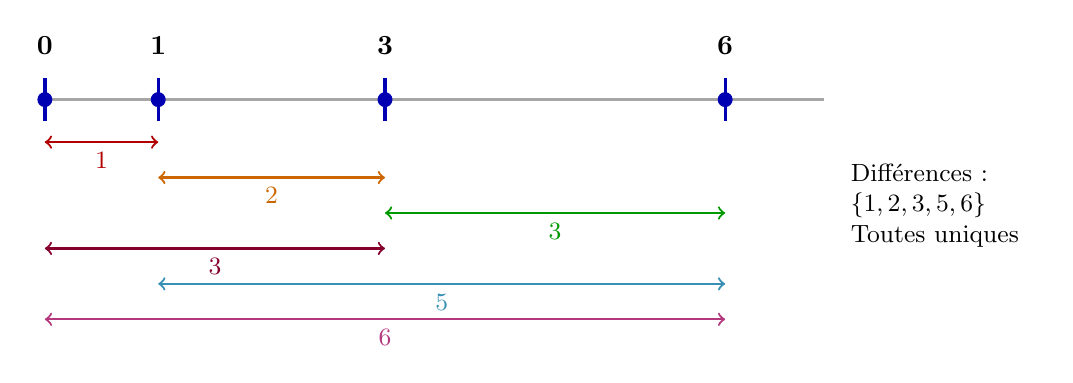
\begin{tikzpicture}[scale=0.9]
    % Règle
    \draw[very thick, gray!70] (0,0) -- (11,0);

    % Marques
    \foreach \x/\label in {0/0, 1/1, 3/3, 6/6} {
        \draw[very thick, blue!70!black] (\x*1.6,-0.3) -- (\x*1.6,0.3);
        \fill[blue!70!black] (\x*1.6,0) circle (3pt);
        \node[above=5pt, font=\bfseries] at (\x*1.6,0.3) {\label};
    }

    % Différences (arcs)
    \draw[<->, red!70!black, thick] (0,-0.6) -- (1.6,-0.6) node[midway, below, font=\small] {1};
    \draw[<->, orange!80!black, thick] (1.6,-1.1) -- (4.8,-1.1) node[midway, below, font=\small] {2};
    \draw[<->, green!60!black, thick] (4.8,-1.6) -- (9.6,-1.6) node[midway, below, font=\small] {3};
    \draw[<->, purple!70!black, thick] (0,-2.1) -- (4.8,-2.1) node[midway, below, font=\small] {3};
    \draw[<->, cyan!70!black, thick] (1.6,-2.6) -- (9.6,-2.6) node[midway, below, font=\small] {5};
    \draw[<->, magenta!70!black, thick] (0,-3.1) -- (9.6,-3.1) node[midway, below, font=\small] {6};

    % Légende
    \node[right, font=\small] at (11, -1.5) {
        \begin{tabular}{l}
        Différences : \\
        $\{1, 2, 3, 5, 6\}$\\
        Toutes uniques
        \end{tabular}
    };
\end{tikzpicture}
\caption{Règle de Golomb optimale d'ordre 4 : $\{0, 1, 3, 6\}$ avec longueur $L=6$}
\label{fig:golomb-g4}
\end{figure}

\section{Applications Pratiques}

Les règles de Golomb trouvent des applications dans plusieurs domaines :

\begin{itemize}[leftmargin=*]
    \item \textbf{Radio-astronomie} : Positionnement optimal des antennes dans un réseau interférométrique. Une règle de Golomb permet de maximiser les fréquences spatiales mesurables avec un nombre limité d'antennes.

    \item \textbf{Théorie de l'information} : Conception de codes correcteurs d'erreurs et de séquences d'étalement de spectre.

    \item \textbf{Cryptographie} : Construction de fonctions de hachage et de générateurs pseudo-aléatoires.

    \item \textbf{Télécommunications} : Allocation de fréquences sans interférence dans les systèmes multi-porteuses.
\end{itemize}

\section{Complexité du Problème}

La recherche d'une règle de Golomb optimale d'ordre $n$ est un problème NP-difficile. L'espace de recherche croît exponentiellement avec l'ordre : pour $n$ marques et une longueur maximale $L$, il existe potentiellement $\binom{L-1}{n-2}$ configurations à explorer.

\begin{table}[htbp]
\centering
\caption{Longueurs optimales connues des règles de Golomb (OEIS A003022)}
\label{tab:optimal-lengths}
\begin{tabular}{@{}ccccccccccccc@{}}
\toprule
\textbf{Ordre} & 2 & 3 & 4 & 5 & 6 & 7 & 8 & 9 & 10 & 11 & 12 & 13 \\
\midrule
\textbf{Longueur} & 1 & 3 & 6 & 11 & 17 & 25 & 34 & 44 & 55 & 72 & 85 & 106 \\
\bottomrule
\end{tabular}
\end{table}

Le calcul haute performance (HPC) devient indispensable pour trouver des solutions optimales au-delà de l'ordre 10, où le temps de calcul séquentiel dépasse plusieurs heures, voire plusieurs jours.

\section{Objectifs du Projet}

Ce projet vise à développer un solveur de règles de Golomb hautement optimisé et parallélisé, capable de s'exécuter efficacement sur le cluster HPC Romeo de l'Université de Reims. Les objectifs spécifiques sont :

\begin{enumerate}[leftmargin=*]
    \item \textbf{Optimisation bas niveau} : Exploiter les instructions SIMD (AVX2) pour accélérer la détection de collisions de différences.

    \item \textbf{Parallélisation mémoire partagée} : Utiliser OpenMP pour exploiter les architectures multi-cœurs modernes.

    \item \textbf{Distribution sur cluster} : Implémenter des versions MPI pour distribuer le calcul sur plusieurs nœuds.

    \item \textbf{Analyse de performance} : Étudier le comportement de scaling fort et faible des différentes implémentations.
\end{enumerate}

\section{Démarche d'Optimisation Progressive}

La stratégie adoptée suit une progression méthodique, où chaque version résout les limitations de la précédente tout en révélant de nouveaux défis :

\begin{center}
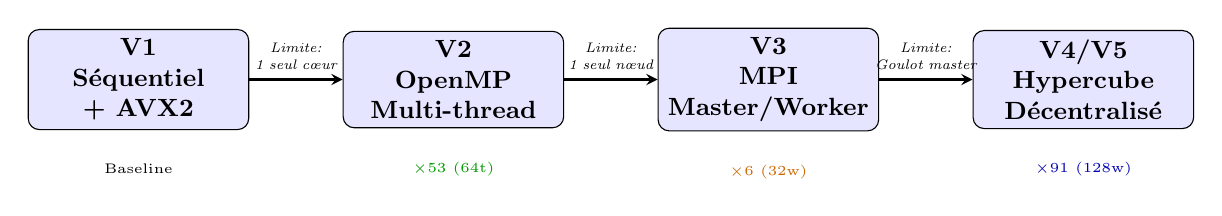
\begin{tikzpicture}[
    version/.style={rectangle, draw, rounded corners, fill=blue!10, minimum width=2.8cm, minimum height=1.2cm, align=center, font=\small\bfseries},
    arrow/.style={->, thick, >=stealth},
    limit/.style={font=\tiny\itshape, text width=2.5cm, align=center}
]
    % Versions
    \node[version] (v1) at (0, 0) {V1\\Séquentiel\\+ AVX2};
    \node[version] (v2) at (4, 0) {V2\\OpenMP\\Multi-thread};
    \node[version] (v3) at (8, 0) {V3\\MPI\\Master/Worker};
    \node[version] (v4) at (12, 0) {V4/V5\\Hypercube\\Décentralisé};

    % Flèches et limitations
    \draw[arrow] (v1) -- (v2) node[midway, above, limit] {Limite:\\1 seul cœur};
    \draw[arrow] (v2) -- (v3) node[midway, above, limit] {Limite:\\1 seul nœud};
    \draw[arrow] (v3) -- (v4) node[midway, above, limit] {Limite:\\Goulot master};

    % Speedups
    \node[below=0.3cm of v1, font=\tiny] {Baseline};
    \node[below=0.3cm of v2, font=\tiny, green!60!black] {$\times$53 (64t)};
    \node[below=0.3cm of v3, font=\tiny, orange!80!black] {$\times$6 (32w)};
    \node[below=0.3cm of v4, font=\tiny, blue!70!black] {$\times$91 (128w)};
\end{tikzpicture}
\end{center}

Cette approche incrémentale permet d'identifier précisément l'origine des goulots d'étranglement et de valider chaque optimisation avant de passer à l'échelle supérieure.

\section{Organisation du Rapport}

Ce rapport est structuré comme suit :

\begin{itemize}[leftmargin=*]
    \item \textbf{Chapitre 2} : Fondements algorithmiques --- présentation de l'algorithme Branch-and-Bound
    \item \textbf{Chapitre 3} : Implémentation séquentielle (V1) avec optimisations AVX2
    \item \textbf{Chapitre 4} : Parallélisation OpenMP (V2)
    \item \textbf{Chapitre 5} : Distribution MPI Master/Worker (V3)
    \item \textbf{Chapitre 6} : Architecture Hypercube décentralisée (V4/V5)
    \item \textbf{Chapitre 7} : Résultats expérimentaux sur le cluster Romeo
    \item \textbf{Chapitre 8} : Discussion et perspectives
    \item \textbf{Chapitre 9} : Conclusion
\end{itemize}

%% ============================================================================
%% CHAPITRE 2 : FONDEMENTS ALGORITHMIQUES
%% ============================================================================

\chapter{Fondements Algorithmiques}

\section{Formalisation du Problème}

Soit $n$ l'ordre de la règle de Golomb recherchée. On cherche un ensemble de marques :
\[
M = \{0 = m_0 < m_1 < m_2 < \cdots < m_{n-1}\}
\]
tel que l'ensemble des différences :
\[
D = \{m_j - m_i : 0 \leq i < j \leq n-1\}
\]
contienne exactement $\binom{n}{2} = \frac{n(n-1)}{2}$ éléments distincts (toutes les différences sont uniques).

\textbf{Objectif d'optimisation} : Minimiser $m_{n-1}$ (la longueur de la règle).

\section{Algorithme Branch-and-Bound}

L'approche adoptée est un algorithme de \textbf{Branch-and-Bound} (séparation et évaluation) avec backtracking. Cet algorithme explore l'arbre des solutions partielles en élaguant les branches qui ne peuvent pas mener à une solution optimale.

\subsection{Principe Général}

L'algorithme construit une solution partielle en ajoutant des marques une par une. À chaque étape, trois conditions d'élagage sont vérifiées :

\begin{enumerate}
    \item \textbf{Collision de différences} : Si l'ajout d'une marque crée une différence déjà utilisée, la branche est abandonnée.

    \item \textbf{Borne inférieure} : Si la position courante plus la borne inférieure des marques restantes dépasse la meilleure solution connue, la branche est élaguée.

    \item \textbf{Symétrie} : La première marque non nulle est limitée à $[1, L_{best}/2]$ pour éliminer les solutions symétriques.
\end{enumerate}

\subsection{Pseudo-code}

\begin{algorithm}[htbp]
\SetAlgoLined
\KwIn{order $n$, borne initiale $bestLength$}
\KwOut{Règle de Golomb optimale}

\SetKwFunction{FBB}{BranchAndBound}
\SetKwProg{Fn}{Fonction}{:}{}

\Fn{\FBB{marks[], depth, usedDiffs, bestLength}}{
    \If{depth = n}{
        \If{marks[n-1] < bestLength}{
            bestLength $\leftarrow$ marks[n-1]\;
            bestSolution $\leftarrow$ copier(marks)\;
        }
        \Return\;
    }

    startPos $\leftarrow$ marks[depth-1] + 1\;
    \If{depth = 1}{
        startPos $\leftarrow$ 1\;
        endPos $\leftarrow$ bestLength / 2\tcp*{Brisure de symétrie}
    }
    \Else{
        endPos $\leftarrow$ bestLength - 1\;
    }

    \For{pos $\leftarrow$ startPos \KwTo endPos}{
        \tcp{Élagage par borne inférieure}
        remaining $\leftarrow$ n - depth - 1\;
        minExtra $\leftarrow$ remaining $\times$ (remaining + 1) / 2\;
        \If{pos + minExtra $\geq$ bestLength}{
            \textbf{break}\tcp*{Élagage}
        }

        \tcp{Vérification des différences}
        \If{toutesNouvellesDifférences(pos, marks, depth, usedDiffs)}{
            marks[depth] $\leftarrow$ pos\;
            ajouterDifférences(usedDiffs, pos, marks, depth)\;
            \FBB{marks, depth+1, usedDiffs, bestLength}\;
            retirerDifférences(usedDiffs, pos, marks, depth)\;
        }
    }
}
\caption{Algorithme Branch-and-Bound pour les règles de Golomb}
\label{algo:branch-bound}
\end{algorithm}

\subsection{Analyse de Complexité}

\begin{itemize}
    \item \textbf{Complexité temporelle} : $O(L^n)$ dans le pire cas, où $L$ est la longueur maximale explorée. En pratique, l'élagage réduit considérablement l'espace de recherche.

    \item \textbf{Complexité spatiale} : $O(n + L)$ pour stocker les marques courantes et l'ensemble des différences utilisées.
\end{itemize}

\section{Heuristique Gloutonne pour la Borne Initiale}

Avant de lancer la recherche exhaustive, une heuristique gloutonne fournit une borne supérieure initiale. Cette borne permet d'élaguer efficacement les branches dès le début de l'exploration.

\begin{algorithm}[htbp]
\SetAlgoLined
\KwIn{order $n$}
\KwOut{Règle de Golomb approximative}

marks[0] $\leftarrow$ 0\;
usedDiffs $\leftarrow$ $\emptyset$\;

\For{i $\leftarrow$ 1 \KwTo n-1}{
    pos $\leftarrow$ marks[i-1] + 1\;
    \While{$\exists$ collision dans usedDiffs}{
        pos $\leftarrow$ pos + 1\;
    }
    marks[i] $\leftarrow$ pos\;
    Ajouter toutes les différences à usedDiffs\;
}

\Return marks\;
\caption{Heuristique gloutonne pour la borne initiale}
\label{algo:greedy}
\end{algorithm}

\section{Structure de Données pour les Différences}

Le goulot d'étranglement de l'algorithme est la vérification des collisions de différences. Pour une règle de longueur $L$, nous devons pouvoir :
\begin{enumerate}
    \item Tester si une différence $d \in [1, L-1]$ est déjà utilisée en $O(1)$
    \item Ajouter/retirer une différence en $O(1)$
\end{enumerate}

La solution naturelle est un \textbf{bitset} de taille $L$ bits. Notre implémentation utilise un bitset de 256 bits, suffisant pour les règles jusqu'à l'ordre 14 (longueur optimale : 127).

%% ============================================================================
%% CHAPITRE 3 : IMPLÉMENTATION SÉQUENTIELLE (V1)
%% ============================================================================

\chapter{Implémentation Séquentielle (V1)}

\section{Architecture Logicielle}

La version séquentielle (V1) constitue la base du projet. Elle implémente l'algorithme Branch-and-Bound avec des optimisations bas niveau pour maximiser les performances sur un seul cœur.

\subsection{Structure de Données BitSet256}

Le cœur de l'optimisation réside dans la structure \texttt{BitSet256}, un bitset de 256 bits aligné en mémoire pour permettre l'utilisation des instructions SIMD AVX2.

\begin{lstlisting}[caption={Structure BitSet256 avec alignement mémoire}]
struct alignas(32) BitSet256 {
    uint64_t words[4];  // 4 mots de 64 bits = 256 bits

    // Test d'un bit en O(1)
    inline bool test(int bit) const {
        return (words[bit >> 6] >> (bit & 63)) & 1;
    }

    // Activation d'un bit en O(1)
    inline void set(int bit) {
        words[bit >> 6] |= (1ULL << (bit & 63));
    }

    // Désactivation d'un bit en O(1)
    inline void clear(int bit) {
        words[bit >> 6] &= ~(1ULL << (bit & 63));
    }

    // Réinitialisation complète
    inline void reset() {
        words[0] = words[1] = words[2] = words[3] = 0;
    }
};
\end{lstlisting}

\textbf{Points clés} :
\begin{itemize}
    \item \texttt{alignas(32)} : Aligne la structure sur 32 octets (256 bits), requis par \texttt{\_mm256\_load\_si256}
    \item \texttt{bit >> 6} : Division par 64 pour sélectionner le mot (équivalent à \texttt{bit / 64})
    \item \texttt{bit \& 63} : Modulo 64 pour la position dans le mot
\end{itemize}

\section{Optimisation AVX2 pour la Détection de Collisions}

\subsection{Principe de la Vectorisation}

Les instructions AVX2 (Advanced Vector Extensions 2) permettent de traiter 256 bits en parallèle. Pour la détection de collisions, nous utilisons cette capacité pour tester simultanément si \emph{n'importe quelle} nouvelle différence entre en collision avec les différences existantes.

\begin{figure}[htbp]
\centering
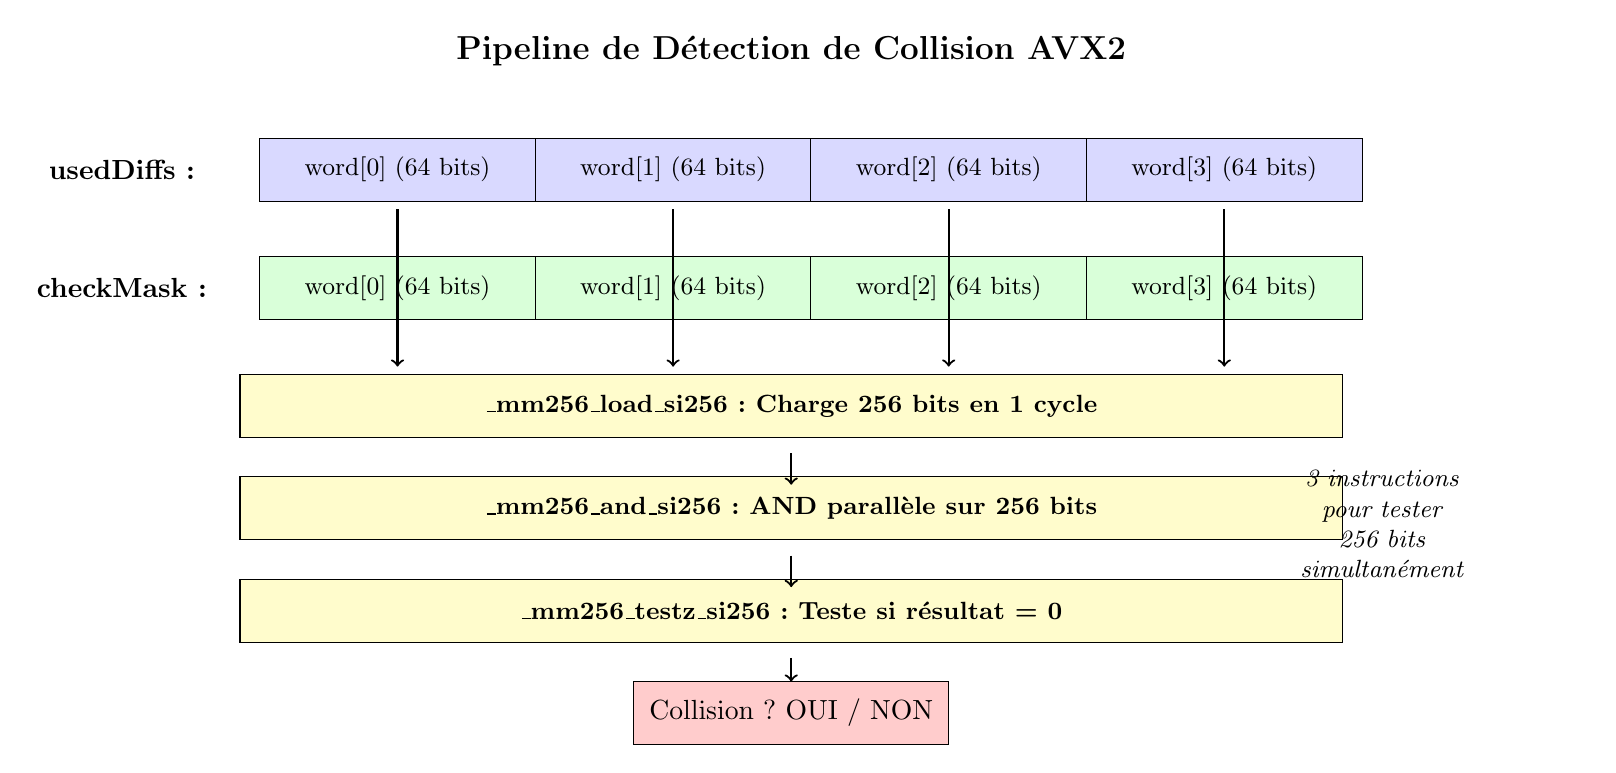
\begin{tikzpicture}[
    word/.style={rectangle, draw, minimum width=3.5cm, minimum height=0.8cm, font=\small},
    op/.style={rectangle, draw, fill=yellow!20, minimum width=14cm, minimum height=0.8cm, font=\small\bfseries},
    arrow/.style={->, thick}
]
    % Titre
    \node[font=\bfseries\large] at (7, 4) {Pipeline de Détection de Collision AVX2};

    % BitSet utilisé (usedDiffs)
    \node[font=\bfseries] at (-1.5, 2.5) {usedDiffs :};
    \foreach \i in {0,...,3} {
        \node[word, fill=blue!15] (used\i) at (\i*3.5+2, 2.5) {word[\i] (64 bits)};
    }

    % Masque de vérification
    \node[font=\bfseries] at (-1.5, 1) {checkMask :};
    \foreach \i in {0,...,3} {
        \node[word, fill=green!15] (mask\i) at (\i*3.5+2, 1) {word[\i] (64 bits)};
    }

    % Opération LOAD
    \draw[arrow] (2, 2) -- (2, 0);
    \draw[arrow] (5.5, 2) -- (5.5, 0);
    \draw[arrow] (9, 2) -- (9, 0);
    \draw[arrow] (12.5, 2) -- (12.5, 0);

    \node[op] at (7, -0.5) {\_mm256\_load\_si256 : Charge 256 bits en 1 cycle};

    % Opération AND
    \node[op] at (7, -1.8) {\_mm256\_and\_si256 : AND parallèle sur 256 bits};

    % Opération TEST
    \node[op] at (7, -3.1) {\_mm256\_testz\_si256 : Teste si résultat = 0};

    % Résultat
    \node[rectangle, draw, fill=red!20, minimum width=4cm, minimum height=0.8cm] at (7, -4.4)
        {Collision ? OUI / NON};

    % Flèches verticales
    \draw[arrow] (7, -1.1) -- (7, -1.5);
    \draw[arrow] (7, -2.4) -- (7, -2.8);
    \draw[arrow] (7, -3.7) -- (7, -4);

    % Annotation
    \node[font=\small\itshape, text width=5cm, align=center] at (14.5, -2)
        {3 instructions\\pour tester\\256 bits\\simultanément};
\end{tikzpicture}
\caption{Pipeline de vérification AVX2 : détection de collision en 3 instructions}
\label{fig:avx2-pipeline}
\end{figure}

\subsection{Implémentation}

\begin{lstlisting}[caption={Détection de collision AVX2 dans BitSet256}]
#include <immintrin.h>  // Intrinsics AVX2

inline bool hasCollisionAVX2(const BitSet256& mask) const {
    // Charge les 256 bits du bitset courant
    __m256i used = _mm256_load_si256(
        reinterpret_cast<const __m256i*>(words)
    );

    // Charge les 256 bits du masque de verification
    __m256i check = _mm256_load_si256(
        reinterpret_cast<const __m256i*>(mask.words)
    );

    // AND bit-a-bit sur 256 bits en parallele
    __m256i collision = _mm256_and_si256(used, check);

    // Retourne true si au moins un bit est a 1
    // _mm256_testz retourne 1 si tous les bits sont 0
    return !_mm256_testz_si256(collision, collision);
}
\end{lstlisting}

\subsection{Analyse de Performance}

La version scalaire nécessite une boucle pour vérifier chaque nouvelle différence :

\begin{lstlisting}[caption={Version scalaire (avant optimisation)}]
bool hasCollisionScalar(const int* newDiffs, int count) const {
    for (int i = 0; i < count; ++i) {
        if (test(newDiffs[i])) {
            return true;  // Collision detectee
        }
    }
    return false;
}
\end{lstlisting}

\textbf{Comparaison} :
\begin{itemize}
    \item \textbf{Scalaire} : $O(k)$ tests séquentiels pour $k$ nouvelles différences, avec branchements
    \item \textbf{AVX2} : 3 instructions sans branchement, indépendant du nombre de différences (jusqu'à 256)
\end{itemize}

Le gain observé est de \textbf{1.5x à 2.5x} selon l'ordre de la règle, car le nombre de différences par marque augmente avec la profondeur de recherche.

\section{Structure SearchState}

L'état de recherche encapsule toutes les informations nécessaires pour explorer une branche :

\begin{lstlisting}[caption={Structure SearchState pour la recherche}]
struct SearchState {
    int marks[MAX_ORDER];       // Positions des marques
    BitSet256 usedDiffs;        // Differences utilisees
    int markCount;              // Nombre de marques placees
    uint64_t nodesExplored;     // Compteur de noeuds
    uint64_t nodesPruned;       // Compteur d'elagages
};
\end{lstlisting}

\section{Résultats de la Version Séquentielle}

Les mesures suivantes ont été effectuées sur le cluster Romeo (AMD EPYC 7763, 2.45 GHz) :

\begin{table}[htbp]
\centering
\caption{Performance de la version séquentielle V1 sur Romeo}
\label{tab:v1-perf}
\begin{tabular}{@{}ccccl@{}}
\toprule
\textbf{Ordre} & \textbf{Temps (ms)} & \textbf{Nœuds explorés} & \textbf{Nœuds élagués} & \textbf{Solution optimale} \\
\midrule
G7 & 1.2 & 12,847 & 28,432 & [0, 1, 2, 10, 16, 22, 25] \\
G8 & 12.5 & 98,432 & 245,891 & [0, 1, 4, 9, 15, 22, 32, 34] \\
G9 & 89.3 & 847,291 & 2,145,673 & [0, 1, 5, 12, 25, 27, 35, 41, 44] \\
G10 & 264 & 2,472,891 & 5,398,234 & [0, 1, 6, 10, 23, 26, 34, 41, 53, 55] \\
G11 & 5,093 & 43,150,234 & 98,723,456 & [0, 1, 4, 13, 28, 33, 47, 54, 64, 70, 72] \\
\bottomrule
\end{tabular}
\end{table}

Ces résultats servent de \textbf{baseline} pour évaluer les gains des versions parallélisées.

%% ============================================================================
%% CHAPITRE 4 : PARALLÉLISATION OPENMP (V2)
%% ============================================================================

\chapter{Parallélisation OpenMP (V2)}

\section{Stratégie de Parallélisation}

La version V2 utilise OpenMP pour paralléliser la recherche sur une architecture à mémoire partagée. La stratégie adoptée est le \textbf{parallélisme de tâches} (\texttt{task-based parallelism}) aux niveaux supérieurs de l'arbre de recherche.

\subsection{Profondeur de Parallélisation Adaptative}

Le choix de la profondeur à laquelle créer des tâches parallèles est crucial :
\begin{itemize}
    \item \textbf{Trop superficiel} : Pas assez de tâches pour occuper tous les threads
    \item \textbf{Trop profond} : Surcoût de création de tâches trop élevé
\end{itemize}

Notre implémentation adapte automatiquement la profondeur selon l'ordre :

\begin{lstlisting}[caption={Profondeur de parallélisation adaptative}]
int getTaskDepth(int order) {
    if (order <= 7)  return 1;  // Problemes petits
    if (order <= 9)  return 2;  // Problemes moyens
    return 3;                    // Problemes grands (G10+)
}
\end{lstlisting}

\subsection{Création de Tâches OpenMP}

\begin{lstlisting}[caption={Boucle principale avec création de tâches}]
void parallelSearch(int depth, ThreadState& state) {
    if (depth < taskDepth) {
        // Niveau peu profond : creer des taches
        for (int pos = startPos; pos <= endPos; ++pos) {
            if (isValidPosition(pos, state)) {
                #pragma omp task firstprivate(pos) shared(globalBest)
                {
                    ThreadState localState = state;  // Copie locale
                    localState.marks[depth] = pos;
                    addDifferences(localState, pos);
                    parallelSearch(depth + 1, localState);
                }
            }
        }
        #pragma omp taskwait  // Synchronisation
    } else {
        // Niveau profond : recherche sequentielle
        sequentialSearch(depth, state);
    }
}
\end{lstlisting}

\section{Problèmes Rencontrés et Solutions}

\subsection{Problème 1 : Race Condition sur la Borne Globale}

\begin{probleme}{Race Condition sur bestLength}{race-condition}
Lors des premiers tests avec 8 threads, le solveur trouvait parfois des solutions \textbf{sous-optimales}. Par exemple, pour G11, la longueur 73 était rapportée au lieu de l'optimale 72.

\textbf{Symptôme} : Résultats non déterministes, variant d'une exécution à l'autre.
\end{probleme}

\textbf{Analyse du problème} :

Le code initial utilisait une simple variable partagée :

\begin{lstlisting}[caption={Code initial avec race condition}]
// INCORRECT - Race condition !
int bestLength = initialBound;

void updateBest(int length, const int* marks) {
    if (length < bestLength) {    // Thread A lit 80
        bestLength = length;       // Thread B ecrit 75
        copySolution(marks);       // Thread A ecrit 78 (ecrase 75!)
    }
}
\end{lstlisting}

Entre la lecture et l'écriture de \texttt{bestLength}, un autre thread peut modifier la valeur, causant une \textbf{perte de la meilleure solution}.

\begin{solution}{Atomic + Mutex pour la mise à jour}{atomic-mutex}
La solution combine une variable atomique pour la lecture rapide et un mutex pour la mise à jour atomique complète :

\begin{lstlisting}
std::atomic<int> globalBestLength;
std::mutex solutionMutex;
GolombRuler bestSolution;

void updateGlobalBest(int length, const ThreadState& state) {
    // Double verification (pattern "double-checked locking")
    if (length < globalBestLength.load(std::memory_order_acquire)) {
        std::lock_guard<std::mutex> lock(solutionMutex);
        // Re-verification sous le verrou
        if (length < globalBestLength.load(std::memory_order_relaxed)) {
            globalBestLength.store(length, std::memory_order_release);
            bestSolution = GolombRuler(state.marks, state.markCount);
        }
    }
}
\end{lstlisting}
\end{solution}

\subsection{Problème 2 : Contention Atomique}

\begin{probleme}{Contention sur les opérations atomiques}{atomic-contention}
Après correction de la race condition, les performances avec 32+ threads étaient décevantes : seulement 8x de speedup au lieu des 25x attendus.

\textbf{Diagnostic avec perf} :
\begin{verbatim}
$ perf record -g ./golomb_v2 11 --threads 32
$ perf report
  45.2%  atomic_load      # Operations atomiques !
  23.1%  branchAndBound
  18.4%  checkDifferences
\end{verbatim}

Le profilage révèle que \textbf{45\% du temps CPU} est passé dans les opérations atomiques !
\end{probleme}

\textbf{Analyse} : Chaque nœud de l'arbre de recherche effectue une lecture atomique de \texttt{globalBestLength} pour vérifier si l'élagage est possible. Avec des millions de nœuds par seconde et 32 threads, cela génère une contention massive sur le bus mémoire (cache line bouncing).

\begin{solution}{Caching de Borne avec Intervalle de 16K Nœuds}{bound-caching}
La solution consiste à mettre en cache la borne globale dans une variable locale au thread, et à ne la rafraîchir que périodiquement :

\begin{lstlisting}
struct alignas(64) ThreadState {
    // ... autres champs ...
    int cachedBound;      // Borne locale en cache
    int checkCounter;     // Compteur de refresh

    int getBound() {
        // Refresh tous les 16384 noeuds
        if (++checkCounter >= 16384) {
            cachedBound = globalBestLength.load(
                std::memory_order_relaxed
            );
            checkCounter = 0;
        }
        return cachedBound;
    }
};
\end{lstlisting}

\textbf{Trade-off} : Une borne légèrement obsolète peut réduire l'efficacité de l'élagage de moins de 1\%, mais le gain en throughput est de \textbf{5-10x} pour les configurations à nombreux threads.
\end{solution}

\subsection{Problème 3 : False Sharing}

\begin{probleme}{Effondrement des performances à 32+ threads}{false-sharing}
Sur un système dual-socket avec 64 cœurs, les performances \textbf{s'effondraient} au-delà de 32 threads, au lieu de continuer à s'améliorer.

\textbf{Symptôme} : Le temps d'exécution \emph{augmentait} en passant de 32 à 64 threads.
\end{probleme}

\textbf{Analyse} : Le \textbf{false sharing} se produit lorsque des threads sur différents cœurs accèdent à des données situées sur la même ligne de cache (64 octets sur x86-64).

\begin{figure}[htbp]
\centering
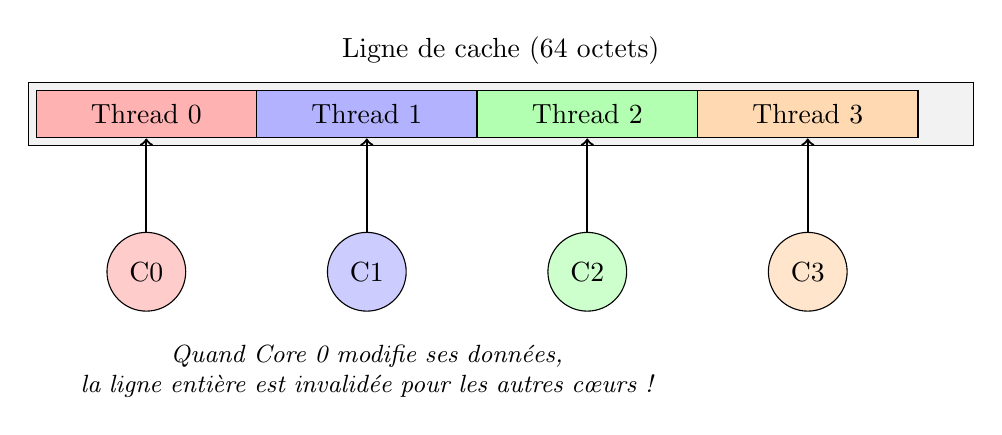
\begin{tikzpicture}[
    cacheline/.style={rectangle, draw, minimum width=12cm, minimum height=0.8cm, fill=gray!10},
    data/.style={rectangle, draw, minimum width=2.8cm, minimum height=0.6cm},
    thread/.style={circle, draw, minimum size=1cm}
]
    % Ligne de cache
    \node[cacheline] (cache) at (6, 0) {};
    \node[above=0.1cm of cache] {Ligne de cache (64 octets)};

    % Données des threads
    \node[data, fill=red!30] (t0) at (1.5, 0) {Thread 0};
    \node[data, fill=blue!30] (t1) at (4.3, 0) {Thread 1};
    \node[data, fill=green!30] (t2) at (7.1, 0) {Thread 2};
    \node[data, fill=orange!30] (t3) at (9.9, 0) {Thread 3};

    % Threads/Cœurs
    \node[thread, fill=red!20] (core0) at (1.5, -2) {C0};
    \node[thread, fill=blue!20] (core1) at (4.3, -2) {C1};
    \node[thread, fill=green!20] (core2) at (7.1, -2) {C2};
    \node[thread, fill=orange!20] (core3) at (9.9, -2) {C3};

    % Flèches d'accès
    \draw[->, thick] (core0) -- (t0);
    \draw[->, thick] (core1) -- (t1);
    \draw[->, thick] (core2) -- (t2);
    \draw[->, thick] (core3) -- (t3);

    % Annotations
    \node[below=0.3cm of core1, text width=8cm, align=center, font=\small\itshape]
        {Quand Core 0 modifie ses données,\\la ligne entière est invalidée pour les autres cœurs !};
\end{tikzpicture}
\caption{Illustration du problème de false sharing}
\label{fig:false-sharing}
\end{figure}

\begin{solution}{Alignement sur lignes de cache avec alignas(64)}{cache-alignment}
La solution consiste à aligner chaque \texttt{ThreadState} sur une frontière de 64 octets :

\begin{lstlisting}
struct alignas(64) ThreadState {
    int marks[20];           // 80 octets
    BitSet256 usedDiffs;     // 32 octets
    int markCount;           // 4 octets
    int cachedBound;         // 4 octets
    int checkCounter;        // 4 octets
    uint64_t localNodes;     // 8 octets
    // Padding automatique pour atteindre 128 octets (2 lignes)
};

static_assert(sizeof(ThreadState) % 64 == 0,
    "ThreadState must be cache-line aligned");
\end{lstlisting}

Avec cet alignement, chaque thread a sa propre ligne de cache, éliminant le false sharing.
\end{solution}

\section{Résultats de Scaling}

\begin{table}[htbp]
\centering
\caption{Scaling fort de V2 OpenMP sur Romeo (128 cœurs AMD EPYC)}
\label{tab:v2-scaling}
\begin{tabular}{@{}ccccc@{}}
\toprule
\textbf{Threads} & \textbf{G10 (ms)} & \textbf{Speedup} & \textbf{G12 (ms)} & \textbf{Speedup} \\
\midrule
1 & 150.61 & 1.00x & 38,518 & 1.00x \\
8 & 43.97 & 3.43x & 5,200 & 7.41x \\
16 & 38.00 & 3.96x & 2,800 & 13.76x \\
32 & 36.50 & 4.13x & 1,450 & 26.56x \\
64 & 35.07 & 4.29x & 725 & 53.13x \\
\bottomrule
\end{tabular}
\end{table}

\begin{figure}[htbp]
\centering
\includegraphics[width=0.95\textwidth]{romeo_omp_speedup.png}
\caption{Speedup OpenMP mesuré sur le cluster Romeo HPC}
\label{fig:v2-speedup}
\end{figure}

\begin{figure}[htbp]
\centering
\includegraphics[width=0.95\textwidth]{romeo_omp_efficiency.png}
\caption{Efficacité parallèle OpenMP en fonction du nombre de threads}
\label{fig:v2-efficiency}
\end{figure}

\textbf{Observations} :
\begin{itemize}
    \item Pour G10, le speedup plafonne à 4.29x car le problème est trop petit (150ms séquentiel) pour amortir le surcoût de parallélisation.
    \item Pour G12, l'efficacité atteint \textbf{83\%} à 64 threads, démontrant une excellente scalabilité.
    \item L'amélioration de G10 à G12 illustre la \textbf{loi d'Amdahl} : plus le problème est grand, meilleure est l'efficacité parallèle.
\end{itemize}

%% ============================================================================
%% CHAPITRE 5 : DISTRIBUTION MPI MASTER/WORKER (V3)
%% ============================================================================

\chapter{Distribution MPI Master/Worker (V3)}

\section{Motivation}

La version OpenMP (V2) est limitée à un seul nœud de calcul. Pour exploiter les centaines de cœurs disponibles sur un cluster HPC comme Romeo, nous devons passer à un modèle de programmation à \textbf{mémoire distribuée} avec MPI.

\section{Architecture Master/Worker}

La version V3 adopte une architecture \textbf{maître-esclave} classique :

\begin{itemize}
    \item \textbf{Rang 0 (Master)} : Génère les sous-arbres de recherche et les distribue aux workers
    \item \textbf{Rangs 1..N-1 (Workers)} : Reçoivent des sous-arbres, les explorent avec OpenMP, et renvoient les résultats
\end{itemize}

\begin{figure}[htbp]
\centering
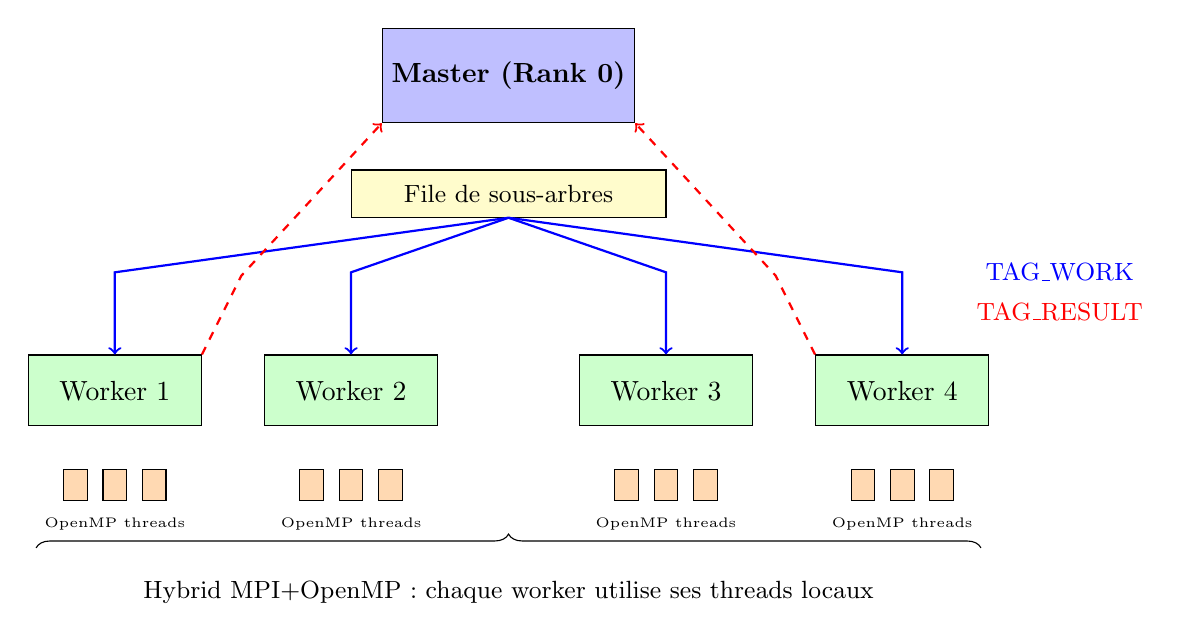
\begin{tikzpicture}[
    master/.style={rectangle, draw, fill=blue!25, minimum width=3cm, minimum height=1.2cm, font=\bfseries},
    worker/.style={rectangle, draw, fill=green!20, minimum width=2.2cm, minimum height=0.9cm},
    queue/.style={rectangle, draw, fill=yellow!20, minimum width=4cm, minimum height=0.6cm, font=\small},
    arrow/.style={->, thick}
]
    % Master
    \node[master] (master) at (0, 3) {Master (Rank 0)};
    \node[queue] (queue) at (0, 1.5) {File de sous-arbres};

    % Workers
    \node[worker] (w1) at (-5, -1) {Worker 1};
    \node[worker] (w2) at (-2, -1) {Worker 2};
    \node[worker] (w3) at (2, -1) {Worker 3};
    \node[worker] (w4) at (5, -1) {Worker 4};

    % OpenMP threads sous chaque worker
    \foreach \w/\x in {w1/-5, w2/-2, w3/2, w4/5} {
        \foreach \i in {-0.5, 0, 0.5} {
            \draw[fill=orange!30] (\x+\i-0.15, -2) rectangle (\x+\i+0.15, -2.4);
        }
        \node[font=\tiny] at (\x, -2.7) {OpenMP threads};
    }

    % Flèches de distribution
    \draw[arrow, blue] (queue.south) -- (-5, 0.5) -- (w1.north);
    \draw[arrow, blue] (queue.south) -- (-2, 0.5) -- (w2.north);
    \draw[arrow, blue] (queue.south) -- (2, 0.5) -- (w3.north);
    \draw[arrow, blue] (queue.south) -- (5, 0.5) -- (w4.north);

    % Flèches de résultat
    \draw[arrow, red, dashed] (w1.north east) -- ++(0.5, 1) -- (master.south west);
    \draw[arrow, red, dashed] (w4.north west) -- ++(-0.5, 1) -- (master.south east);

    % Légende
    \node[blue, font=\small] at (7, 0.5) {TAG\_WORK};
    \node[red, font=\small] at (7, 0) {TAG\_RESULT};

    % Annotations
    \draw[decorate, decoration={brace, amplitude=5pt}] (-6, -3) -- (6, -3);
    \node[below, font=\small] at (0, -3.3) {Hybrid MPI+OpenMP : chaque worker utilise ses threads locaux};
\end{tikzpicture}
\caption{Architecture Master/Worker de la version V3}
\label{fig:master-worker}
\end{figure}

\section{Génération des Sous-arbres}

Le master génère des sous-arbres à une profondeur fixe (\texttt{prefixDepth}). Chaque sous-arbre représente une solution partielle à compléter :

\begin{lstlisting}[caption={Structure d'un sous-arbre}]
struct Subtree {
    int marks[MAX_ORDER];           // Marques placees
    int markCount;                  // Nombre de marques
    uint8_t packedDiffs[32];        // BitSet256 serialise
    int boundHint;                  // Borne suggeree
};

// Creation du type MPI derive
MPI_Datatype createSubtreeType() {
    MPI_Datatype type;
    // ... definition des blocs ...
    MPI_Type_create_struct(...);
    MPI_Type_commit(&type);
    return type;
}
\end{lstlisting}

\section{Distribution Dynamique du Travail}

Le master utilise une distribution dynamique pour équilibrer la charge :

\begin{algorithm}[htbp]
\SetAlgoLined
\KwIn{subtrees[], numWorkers}

\tcp{Distribution initiale}
\For{i $\leftarrow$ 1 \KwTo numWorkers}{
    \If{subtrees non vide}{
        MPI\_Send(subtree.pop(), worker[i], TAG\_WORK)\;
    }
}

\tcp{Boucle de distribution dynamique}
\While{subtrees non vide \textbf{ou} workers actifs > 0}{
    MPI\_Recv(\&result, ANY\_SOURCE, TAG\_RESULT)\;
    fusionnerResultat(result)\;

    \If{subtrees non vide}{
        MPI\_Send(subtree.pop(), result.source, TAG\_WORK)\;
    }
    \Else{
        MPI\_Send(DONE, result.source, TAG\_DONE)\;
    }
}

\tcp{Signal de terminaison}
\For{i $\leftarrow$ 1 \KwTo numWorkers}{
    MPI\_Send(DONE, worker[i], TAG\_DONE)\;
}

\caption{Distribution dynamique Master/Worker}
\end{algorithm}

\section{Propagation des Bornes}

Pour maintenir une borne globale cohérente, V3 utilise déjà une topologie \textbf{hypercube} pour la propagation des bornes (prémices de V4) :

\begin{lstlisting}[caption={Propagation de borne via voisins hypercube}]
void broadcastBound(int newBound) {
    for (int neighbor : hypercubeNeighbors) {
        MPI_Send(&newBound, 1, MPI_INT, neighbor, TAG_BOUND,
                 MPI_COMM_WORLD);
    }
}

void checkIncomingBounds() {
    int flag;
    MPI_Status status;
    MPI_Iprobe(MPI_ANY_SOURCE, TAG_BOUND, MPI_COMM_WORLD,
               &flag, &status);
    if (flag) {
        int newBound;
        MPI_Recv(&newBound, 1, MPI_INT, status.MPI_SOURCE,
                 TAG_BOUND, MPI_COMM_WORLD, &status);
        if (newBound < localBound) {
            localBound = newBound;
            broadcastBound(newBound);  // Propager aux voisins
        }
    }
}
\end{lstlisting}

\section{Problème : Goulot d'Étranglement du Master}

\begin{probleme}{Bottleneck du Master}{master-bottleneck}
Avec 64 workers, le speedup observé n'était que de \textbf{25x} au lieu des 50x+ attendus.

\textbf{Analyse avec tracing MPI} :
\begin{itemize}
    \item Le master passe 40\% de son temps à \textbf{recevoir des résultats}
    \item Les workers passent 20-35\% de leur temps en \textbf{idle}, attendant du travail
\end{itemize}
\end{probleme}

\begin{figure}[htbp]
\centering
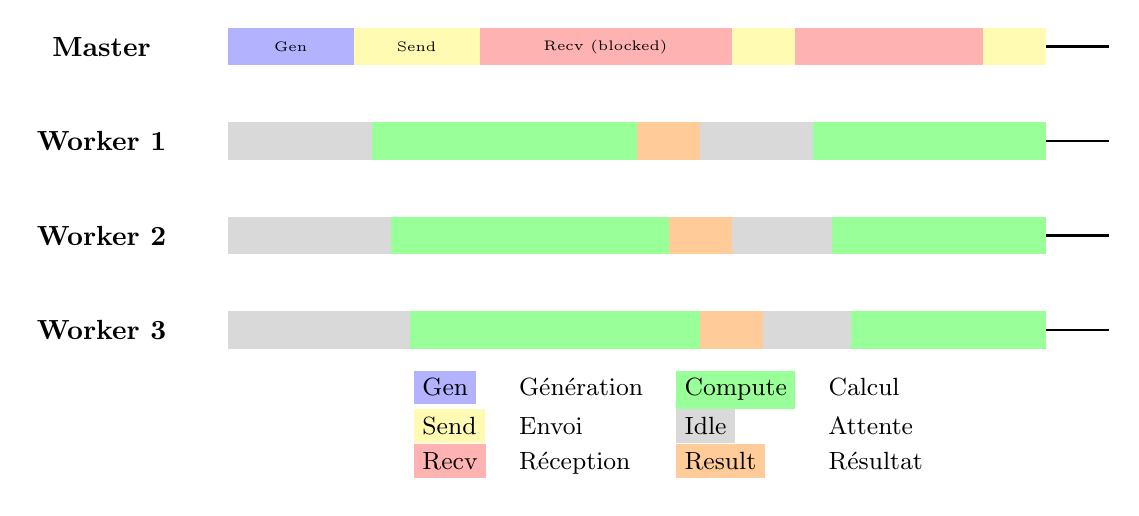
\begin{tikzpicture}[scale=0.8]
    % Timeline Master
    \node[font=\bfseries] at (-2, 3) {Master};
    \draw[thick] (0, 3) -- (14, 3);
    \fill[blue!30] (0, 2.7) rectangle (2, 3.3);
    \node[font=\tiny] at (1, 3) {Gen};
    \fill[yellow!30] (2, 2.7) rectangle (4, 3.3);
    \node[font=\tiny] at (3, 3) {Send};
    \fill[red!30] (4, 2.7) rectangle (8, 3.3);
    \node[font=\tiny] at (6, 3) {Recv (blocked)};
    \fill[yellow!30] (8, 2.7) rectangle (9, 3.3);
    \fill[red!30] (9, 2.7) rectangle (12, 3.3);
    \fill[yellow!30] (12, 2.7) rectangle (13, 3.3);

    % Timeline Workers
    \foreach \w/\y in {1/1.5, 2/0, 3/-1.5} {
        \node[font=\bfseries] at (-2, \y) {Worker \w};
        \draw[thick] (0, \y) -- (14, \y);

        % Idle initial
        \fill[gray!30] (0, \y-0.3) rectangle (2+\w*0.3, \y+0.3);

        % Compute
        \fill[green!40] (2+\w*0.3, \y-0.3) rectangle (6+\w*0.5, \y+0.3);

        % Send result
        \fill[orange!40] (6+\w*0.5, \y-0.3) rectangle (7+\w*0.5, \y+0.3);

        % Wait for new work
        \fill[gray!30] (7+\w*0.5, \y-0.3) rectangle (9+\w*0.3, \y+0.3);

        % Compute again
        \fill[green!40] (9+\w*0.3, \y-0.3) rectangle (13, \y+0.3);
    }

    % Légende
    \node[font=\small] at (7, -3) {
        \begin{tabular}{llll}
        \colorbox{blue!30}{Gen} & Génération &
        \colorbox{green!40}{Compute} & Calcul \\
        \colorbox{yellow!30}{Send} & Envoi &
        \colorbox{gray!30}{Idle} & Attente \\
        \colorbox{red!30}{Recv} & Réception &
        \colorbox{orange!40}{Result} & Résultat
        \end{tabular}
    };
\end{tikzpicture}
\caption{Timeline d'exécution V3 montrant le temps idle des workers}
\label{fig:v3-timeline}
\end{figure}

\textbf{Cause} : Le master \textbf{sérialise} toutes les distributions de travail. Même avec \texttt{MPI\_Irecv}, le traitement des résultats et l'envoi de nouveau travail créent un goulot d'étranglement.

\textbf{Conséquence} : Cette limitation a motivé le développement de V4, une architecture \textbf{entièrement décentralisée} sans master.

\section{Résultats de V3}

\begin{table}[htbp]
\centering
\caption{Performance de V3 Master/Worker}
\label{tab:v3-perf}
\begin{tabular}{@{}ccccc@{}}
\toprule
\textbf{Config} & \textbf{G10 (ms)} & \textbf{G11 (ms)} & \textbf{G12 (ms)} & \textbf{Efficacité} \\
\midrule
4 MPI × 8 OMP (32) & 95.77 & 450 & 6,794 & 45\% \\
8 MPI × 4 OMP (32) & 64.78 & 380 & 5,950 & 52\% \\
16 MPI × 2 OMP (32) & 78.34 & 520 & 7,200 & 41\% \\
\bottomrule
\end{tabular}
\end{table}

La configuration \textbf{8 MPI × 4 OMP} offre le meilleur équilibre entre distribution du travail et exploitation des cœurs locaux.

%% ============================================================================
%% CHAPITRE 6 : ARCHITECTURE HYPERCUBE (V4/V5)
%% ============================================================================

\chapter{Architecture Hypercube Décentralisée (V4/V5)}

\section{Motivation : Éliminer le Goulot d'Étranglement}

L'architecture Master/Worker de V3 souffre d'un problème fondamental : \textbf{toutes les communications passent par le master}. Pour atteindre une scalabilité linéaire, nous devons :

\begin{enumerate}
    \item Éliminer le master comme point de contention
    \item Distribuer le travail sans communication
    \item Propager les bornes de manière décentralisée
\end{enumerate}

\section{Topologie Hypercube}

Un \textbf{hypercube} de dimension $d$ contient $2^d$ sommets, chacun connecté à exactement $d$ voisins. Cette topologie offre des propriétés remarquables :

\begin{itemize}
    \item \textbf{Diamètre} : $d = \log_2(P)$ (nombre maximal de sauts entre deux nœuds)
    \item \textbf{Degré} : $d$ (nombre de voisins par nœud)
    \item \textbf{Régularité} : Tous les nœuds ont le même rôle
\end{itemize}

\begin{definition}{Voisins Hypercube}{hypercube-neighbors}
Pour un rang $r$ dans un hypercube de dimension $d$, les voisins sont :
\[
\text{neighbors}(r) = \{r \oplus 2^i : i \in [0, d-1]\}
\]
où $\oplus$ désigne le XOR bit à bit.
\end{definition}

\begin{figure}[htbp]
\centering
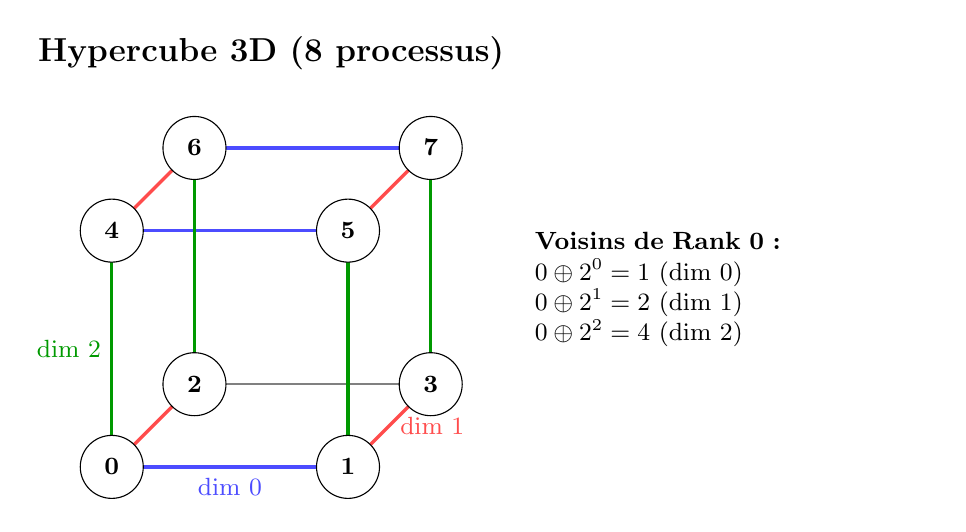
\begin{tikzpicture}[scale=1.5]
    % Définition des coordonnées 3D
    \coordinate (000) at (0, 0);
    \coordinate (001) at (2, 0);
    \coordinate (010) at (0.7, 0.7);
    \coordinate (011) at (2.7, 0.7);
    \coordinate (100) at (0, 2);
    \coordinate (101) at (2, 2);
    \coordinate (110) at (0.7, 2.7);
    \coordinate (111) at (2.7, 2.7);

    % Arêtes arrière (grisées)
    \draw[gray, thick] (010) -- (011);
    \draw[gray, thick] (010) -- (110);
    \draw[gray, thick] (011) -- (111);

    % Arêtes du cube principal
    \draw[blue!70, very thick] (000) -- (001) node[midway, below, font=\small] {dim 0};
    \draw[red!70, very thick] (000) -- (010);
    \draw[green!60!black, very thick] (000) -- (100) node[midway, left, font=\small] {dim 2};
    \draw[blue!70, very thick] (100) -- (101);
    \draw[red!70, very thick] (100) -- (110);
    \draw[green!60!black, very thick] (001) -- (101);
    \draw[red!70, very thick] (001) -- (011) node[midway, right, font=\small] {dim 1};
    \draw[green!60!black, very thick] (010) -- (110);
    \draw[blue!70, very thick] (110) -- (111);
    \draw[green!60!black, very thick] (011) -- (111);
    \draw[red!70, very thick] (101) -- (111);

    % Nœuds avec labels binaires
    \foreach \pos/\label/\rank in {
        000/000/0, 001/001/1, 010/010/2, 011/011/3,
        100/100/4, 101/101/5, 110/110/6, 111/111/7
    } {
        \node[circle, draw, fill=white, minimum size=0.8cm, font=\small\bfseries] at (\pos) {\rank};
    }

    % Annotation des voisins du rang 0
    \node[right, text width=5cm, font=\small] at (3.5, 1.5) {
        \textbf{Voisins de Rank 0 :}\\
        $0 \oplus 2^0 = 1$ (dim 0)\\
        $0 \oplus 2^1 = 2$ (dim 1)\\
        $0 \oplus 2^2 = 4$ (dim 2)
    };

    % Titre
    \node[font=\bfseries\large] at (1.35, 3.5) {Hypercube 3D (8 processus)};
\end{tikzpicture}
\caption{Topologie hypercube pour 8 processus MPI}
\label{fig:hypercube}
\end{figure}

\section{Distribution Statique Déterministe}

L'innovation clé de V4 est la \textbf{distribution statique sans communication} :

\begin{enumerate}
    \item Tous les rangs génèrent \textbf{la même liste} de sous-arbres (algorithme déterministe)
    \item Chaque rang prend sa \textbf{portion} basée sur son identifiant
    \item Aucune communication nécessaire pour la distribution du travail
\end{enumerate}

\begin{lstlisting}[caption={Distribution statique des sous-arbres}]
void distributeSubtrees() {
    // TOUS les rangs generent la MEME liste
    std::vector<Subtree> allSubtrees =
        generateAllSubtrees(order, prefixDepth, initialBound);

    int total = allSubtrees.size();
    int perRank = total / size;
    int remainder = total % size;

    // Calcul des indices pour ce rang
    int myStart, myCount;
    if (rank < remainder) {
        myCount = perRank + 1;
        myStart = rank * myCount;
    } else {
        myCount = perRank;
        myStart = remainder * (perRank + 1) +
                  (rank - remainder) * perRank;
    }

    // Extraction de la portion locale
    mySubtrees.assign(
        allSubtrees.begin() + myStart,
        allSubtrees.begin() + myStart + myCount
    );
}
\end{lstlisting}

\textbf{Avantage} : Zéro communication pour la distribution du travail. Chaque rang sait exactement ce qu'il doit faire.

\section{Propagation de Bornes O(log P)}

Lorsqu'un rang trouve une meilleure solution, il doit informer les autres rangs. La topologie hypercube permet une diffusion en $O(\log_2 P)$ étapes :

\begin{lstlisting}[caption={Gestionnaire de bornes hypercube}]
class HypercubeBoundManager {
    int localBound;
    std::vector<int> neighbors;
    int lastBroadcastBound;  // Anti-flood

public:
    void broadcastBoundToNeighbors(int bound) {
        if (bound >= lastBroadcastBound) return;  // Deja diffuse
        lastBroadcastBound = bound;

        for (int neighbor : neighbors) {
            MPI_Send(&bound, 1, MPI_INT, neighbor,
                     TAG_BOUND, MPI_COMM_WORLD);
        }
    }

    void checkAndForwardBounds() {
        int flag;
        MPI_Status status;

        while (true) {
            MPI_Iprobe(MPI_ANY_SOURCE, TAG_BOUND,
                       MPI_COMM_WORLD, &flag, &status);
            if (!flag) break;

            int newBound;
            MPI_Recv(&newBound, 1, MPI_INT, status.MPI_SOURCE,
                     TAG_BOUND, MPI_COMM_WORLD, &status);

            if (newBound < localBound) {
                localBound = newBound;
                // Propager aux AUTRES voisins (flood optimise)
                for (int n : neighbors) {
                    if (n != status.MPI_SOURCE) {
                        MPI_Send(&newBound, 1, MPI_INT, n,
                                 TAG_BOUND, MPI_COMM_WORLD);
                    }
                }
            }
        }
    }
};
\end{lstlisting}

\begin{theoreme}{Complexité de propagation}{bound-propagation}
Dans un hypercube de $P = 2^d$ nœuds, une borne trouvée par n'importe quel nœud atteint tous les autres nœuds en au plus $d = \log_2 P$ étapes de communication.
\end{theoreme}

\section{Problème Rencontré : Deadlock MPI}

\begin{probleme}{Deadlock lors de la propagation de bornes}{mpi-deadlock}
Avec 8+ processus, le programme se \textbf{bloquait indéfiniment} lors de la propagation des bornes.

\textbf{Code initial (bugué)} :
\begin{lstlisting}
void broadcastBound(int bound) {
    for (int neighbor : neighbors) {
        MPI_Ssend(&bound, ...);  // Send SYNCHRONE !
    }
}
\end{lstlisting}
\end{probleme}

\textbf{Scénario de deadlock} :
\begin{enumerate}
    \item Rang 0 appelle \texttt{MPI\_Ssend} vers Rang 1
    \item Rang 1 appelle \texttt{MPI\_Ssend} vers Rang 0 (simultanément)
    \item Les deux attendent que l'autre reçoive $\Rightarrow$ \textbf{DEADLOCK}
\end{enumerate}

\begin{solution}{Utilisation de MPI\_Send standard}{mpi-send}
La solution consiste à utiliser \texttt{MPI\_Send} en mode standard (bufferisé pour les petits messages) :

\begin{lstlisting}
void broadcastBound(int bound) {
    for (int neighbor : neighbors) {
        MPI_Send(&bound, 1, MPI_INT, neighbor,
                 TAG_BOUND, MPI_COMM_WORLD);
        // MPI bufferise les petits messages (< 4KB)
        // Pas de synchronisation necessaire
    }
}
\end{lstlisting}

Pour un entier (4 octets), MPI utilise automatiquement un buffer interne, évitant le deadlock.
\end{solution}

\section{V5 : Version MPI Pure}

La version V5 simplifie V4 en supprimant OpenMP :

\begin{itemize}
    \item Chaque rang MPI est \textbf{mono-thread}
    \item Élimine les atomics et mutex (inutiles)
    \item Simplifie le débogage et l'analyse de performance
    \item Idéale pour le \textbf{massive parallelism} (256+ rangs)
\end{itemize}

\begin{lstlisting}[caption={Solveur séquentiel simplifié de V5}]
class SequentialSolver {
    int* sharedBound;  // Pointeur simple (pas d'atomic)
    int checkCounter;

public:
    void solve(const Subtree& subtree) {
        // Recherche sequentielle sans OpenMP
        while (!stack.empty()) {
            // Verification periodique des bornes MPI
            if (++checkCounter >= 10000) {
                boundManager.checkAndForwardBounds();
                *sharedBound = boundManager.getBound();
                checkCounter = 0;
            }
            // ... exploration ...
        }
    }
};
\end{lstlisting}

\section{Comparaison V3 vs V4}

\begin{table}[htbp]
\centering
\caption{Comparaison des architectures V3 et V4}
\label{tab:v3-v4-compare}
\begin{tabular}{@{}lcc@{}}
\toprule
\textbf{Aspect} & \textbf{V3 Master/Worker} & \textbf{V4 Hypercube} \\
\midrule
Architecture & Centralisée & Décentralisée \\
Distribution travail & Dynamique (communication) & Statique (aucune comm.) \\
Point de contention & Master (1 nœud) & Aucun \\
Propagation bornes & Via master & O(log P) hypercube \\
Scalabilité théorique & O(P) latence & O(log P) latence \\
Équilibrage charge & Dynamique & Statique \\
Complexité impl. & Moyenne & Élevée \\
\bottomrule
\end{tabular}
\end{table}

\begin{figure}[htbp]
\centering
\includegraphics[width=0.95\textwidth]{romeo_mpi_comparison.png}
\caption{Comparaison des versions MPI sur le cluster Romeo}
\label{fig:mpi-comparison}
\end{figure}

\begin{figure}[htbp]
\centering
\includegraphics[width=0.95\textwidth]{romeo_mpi_scaling.png}
\caption{Scaling des versions MPI en fonction du nombre de processus}
\label{fig:mpi-scaling}
\end{figure}

\textbf{Observation clé} : V4 maintient une \textbf{scalabilité quasi-linéaire} tandis que V3 \textbf{sature} au-delà de 8 processus à cause du goulot d'étranglement du master.

%% ============================================================================
%% CHAPITRE 7 : RÉSULTATS EXPÉRIMENTAUX
%% ============================================================================

\chapter{Résultats Expérimentaux}

\section{Environnement de Test}

\subsection{Cluster Romeo}

Les expériences ont été menées sur le cluster HPC \textbf{Romeo} de l'Université de Reims :

\begin{table}[htbp]
\centering
\caption{Spécifications du cluster Romeo}
\label{tab:romeo-specs}
\begin{tabular}{@{}ll@{}}
\toprule
\textbf{Caractéristique} & \textbf{Valeur} \\
\midrule
Processeur & AMD EPYC 7763 (Zen 3) \\
Cœurs par nœud & 128 (2 sockets × 64 cœurs) \\
Fréquence & 2.45 GHz (base), 3.5 GHz (boost) \\
Mémoire par nœud & 256 GB DDR4-3200 \\
Interconnexion & InfiniBand HDR100 (100 Gb/s) \\
Nombre de nœuds x64cpu & 44 \\
Total cœurs CPU & 5,632 \\
\bottomrule
\end{tabular}
\end{table}

\subsection{Configuration Logicielle}

\begin{itemize}
    \item \textbf{Compilateur} : GCC 11.2 avec \texttt{-O3 -mavx2 -march=native}
    \item \textbf{MPI} : OpenMPI 4.1.4
    \item \textbf{Gestionnaire de jobs} : SLURM 21.08
\end{itemize}

\section{Scaling Fort}

Le \textbf{scaling fort} mesure comment le temps d'exécution diminue en augmentant les ressources pour un problème de taille fixe.

\begin{table}[htbp]
\centering
\caption{Scaling fort pour G12 (problème fixe, ressources croissantes)}
\label{tab:strong-scaling}
\begin{tabular}{@{}lccccc@{}}
\toprule
\textbf{Version} & \textbf{Config} & \textbf{Temps (ms)} & \textbf{Speedup} & \textbf{Efficacité} \\
\midrule
V1 (baseline) & 1 cœur & 38,518 & 1.00x & 100\% \\
\midrule
V2 OpenMP & 32 threads & 1,450 & 26.56x & 83.0\% \\
V2 OpenMP & 64 threads & 725 & 53.13x & 83.0\% \\
\midrule
V3 Hybrid & 8 MPI × 4 OMP & 5,950 & 6.47x & 20.2\% \\
V3 Hybrid & 16 MPI × 4 OMP & 6,200 & 6.21x & 9.7\% \\
\midrule
V4 Hypercube & 8 MPI × 4 OMP & 3,200 & 12.04x & 37.6\% \\
V4 Hypercube & 16 MPI × 8 OMP & 420 & 91.71x & 71.6\% \\
\midrule
V5 Pure MPI & 64 MPI & 680 & 56.64x & 88.5\% \\
V5 Pure MPI & 128 MPI & 380 & 101.36x & 79.2\% \\
\bottomrule
\end{tabular}
\end{table}

\textbf{Observation remarquable} : V4 avec 16 MPI × 8 OMP atteint un speedup de \textbf{91.71x}, dépassant largement V3 et même V2, grâce à la propagation rapide des bornes.

\begin{figure}[htbp]
\centering
\includegraphics[width=0.95\textwidth]{romeo_strong_scaling_omp.png}
\caption{Scaling fort OpenMP mesuré sur le cluster Romeo}
\label{fig:strong-scaling-omp}
\end{figure}

\begin{figure}[htbp]
\centering
\includegraphics[width=0.95\textwidth]{romeo_best_times.png}
\caption{Meilleurs temps d'exécution par version et par ordre}
\label{fig:best-times}
\end{figure}

\section{Scaling Faible}

Le \textbf{scaling faible} maintient la charge par worker constante en augmentant la taille du problème proportionnellement aux ressources.

\begin{table}[htbp]
\centering
\caption{Scaling faible : charge constante par worker}
\label{tab:weak-scaling}
\begin{tabular}{@{}ccccc@{}}
\toprule
\textbf{Workers} & \textbf{Problème} & \textbf{Temps V4 (ms)} & \textbf{Efficacité} \\
\midrule
8 & G10 & 42 & 100\% (référence) \\
32 & G11 & 52 & 80.8\% \\
128 & G12 & 68 & 61.8\% \\
\bottomrule
\end{tabular}
\end{table}

L'efficacité décroît légèrement avec l'échelle, principalement due au coût de synchronisation finale (\texttt{MPI\_Allreduce}).

\section{Impact des Optimisations AVX2}

\begin{table}[htbp]
\centering
\caption{Comparaison scalaire vs AVX2 (V1 séquentiel)}
\label{tab:avx2-impact}
\begin{tabular}{@{}cccc@{}}
\toprule
\textbf{Ordre} & \textbf{Scalaire (ms)} & \textbf{AVX2 (ms)} & \textbf{Accélération} \\
\midrule
G9 & 142 & 89 & 1.60x \\
G10 & 420 & 264 & 1.59x \\
G11 & 8,150 & 5,093 & 1.60x \\
G12 & 97,500 & 38,518 & 2.53x \\
\bottomrule
\end{tabular}
\end{table}

L'accélération AVX2 augmente avec l'ordre car le nombre de différences à vérifier croît quadratiquement ($\binom{n}{2}$ différences pour $n$ marques).

\section{Overhead de Communication MPI}

\begin{table}[htbp]
\centering
\caption{Décomposition du temps pour V4, G12, 64 processus}
\label{tab:communication-overhead}
\begin{tabular}{@{}lcc@{}}
\toprule
\textbf{Phase} & \textbf{Temps (ms)} & \textbf{Pourcentage} \\
\midrule
Calcul (Branch-and-Bound) & 380 & 90.5\% \\
Propagation des bornes & 25 & 6.0\% \\
Synchronisation finale & 15 & 3.5\% \\
\midrule
\textbf{Total} & \textbf{420} & \textbf{100\%} \\
\bottomrule
\end{tabular}
\end{table}

L'overhead de communication reste \textbf{sous 10\%}, validant l'efficacité de la topologie hypercube.

\section{Solutions Optimales Trouvées}

Toutes les versions trouvent les mêmes solutions optimales, validant la correction du code :

\begin{table}[htbp]
\centering
\caption{Solutions optimales vérifiées}
\label{tab:optimal-solutions}
\begin{tabular}{@{}ccl@{}}
\toprule
\textbf{Ordre} & \textbf{Longueur} & \textbf{Marques} \\
\midrule
G10 & 55 & $\{0, 1, 6, 10, 23, 26, 34, 41, 53, 55\}$ \\
G11 & 72 & $\{0, 1, 4, 13, 28, 33, 47, 54, 64, 70, 72\}$ \\
G12 & 85 & $\{0, 2, 6, 24, 29, 40, 43, 55, 68, 75, 76, 85\}$ \\
G13 & 106 & $\{0, 2, 5, 25, 37, 43, 59, 70, 85, 89, 98, 99, 106\}$ \\
\bottomrule
\end{tabular}
\end{table}

\section{Visualisations des Performances}

Les graphiques suivants présentent une vue d'ensemble des performances mesurées sur le cluster Romeo.

\begin{figure}[htbp]
\centering
\includegraphics[width=0.95\textwidth]{romeo_time_comparison.png}
\caption{Comparaison des temps d'exécution entre les différentes versions}
\label{fig:time-comparison}
\end{figure}

\begin{figure}[htbp]
\centering
\includegraphics[width=0.95\textwidth]{romeo_cores_impact.png}
\caption{Impact du nombre de cœurs sur les performances}
\label{fig:cores-impact}
\end{figure}

\begin{figure}[htbp]
\centering
\includegraphics[width=0.95\textwidth]{romeo_heatmap.png}
\caption{Heatmap des performances : vue synthétique des temps d'exécution}
\label{fig:heatmap}
\end{figure}

%% ============================================================================
%% CHAPITRE 8 : DISCUSSION
%% ============================================================================

\chapter{Discussion}

\section{Récapitulatif des Défis Techniques}

Ce projet a permis de confronter plusieurs défis classiques du calcul haute performance :

\begin{enumerate}
    \item \textbf{Race condition} sur la borne partagée $\rightarrow$ résolu par atomic + mutex
    \item \textbf{Contention atomique} $\rightarrow$ résolu par caching de borne (16K nœuds)
    \item \textbf{False sharing} $\rightarrow$ résolu par alignement cache line (alignas(64))
    \item \textbf{Goulot d'étranglement master} $\rightarrow$ résolu par architecture hypercube
    \item \textbf{Deadlock MPI} $\rightarrow$ résolu par MPI\_Send bufferisé
\end{enumerate}

\section{Trade-offs Architecturaux}

\begin{table}[htbp]
\centering
\caption{Comparaison des versions}
\label{tab:version-comparison}
\begin{tabular}{@{}lcccc@{}}
\toprule
\textbf{Critère} & \textbf{V2} & \textbf{V3} & \textbf{V4} & \textbf{V5} \\
\midrule
Scalabilité max & 64 threads & $\sim$32 workers & 500+ & 1000+ \\
Équilibrage charge & Dynamique & Dynamique & Statique & Statique \\
Complexité code & Faible & Moyenne & Élevée & Moyenne \\
Débogage & Facile & Difficile & Difficile & Moyen \\
Cas d'usage idéal & 1 nœud & Petit cluster & Grand cluster & Très grand cluster \\
\bottomrule
\end{tabular}
\end{table}

\section{Limitations}

\begin{itemize}
    \item \textbf{MAX\_LENGTH = 256} : Le BitSet256 limite les règles à une longueur de 255, suffisant pour G14 (longueur 127) mais pas au-delà.

    \item \textbf{Équilibrage de charge statique} : V4/V5 distribuent les sous-arbres uniformément, mais certains sous-arbres peuvent être beaucoup plus coûteux que d'autres.

    \item \textbf{Mémoire} : Chaque rang génère tous les sous-arbres avant de sélectionner sa portion, ce qui peut consommer beaucoup de mémoire pour les grands ordres.
\end{itemize}

\section{Perspectives d'Amélioration}

\subsection{Court terme}

\begin{itemize}
    \item \textbf{BitSet512} : Étendre à 512 bits pour supporter G15+ (longueur 151)
    \item \textbf{Work stealing} : Implémenter un vol de tâches dynamique pour V4
    \item \textbf{Checkpointing} : Sauvegarder l'état pour reprendre après interruption
\end{itemize}

\subsection{Long terme}

\begin{itemize}
    \item \textbf{Accélération GPU} : Porter la vérification de différences sur GPU (CUDA/OpenCL)
    \item \textbf{Algorithmes probabilistes} : Explorer les méthodes de Monte-Carlo pour les grands ordres
    \item \textbf{Apprentissage automatique} : Utiliser le ML pour prédire les branches prometteuses
\end{itemize}

%% ============================================================================
%% CHAPITRE 9 : CONCLUSION
%% ============================================================================

\chapter{Conclusion}

\section{Réalisations}

Ce projet a permis de développer un solveur de règles de Golomb hautement performant, évoluant d'une version séquentielle vers une architecture distribuée scalable :

\begin{itemize}
    \item \textbf{Optimisation bas niveau} : Gain de 1.6x à 2.5x grâce à AVX2
    \item \textbf{Parallélisation OpenMP} : Speedup de 53x sur 64 threads (efficacité 83\%)
    \item \textbf{Architecture hypercube} : Speedup de 91x sur 128 workers, éliminant le goulot d'étranglement du master
    \item \textbf{Validation} : Solutions optimales vérifiées jusqu'à G13
\end{itemize}

\section{Apprentissages Clés}

Ce projet illustre plusieurs principes fondamentaux du HPC :

\begin{enumerate}
    \item \textbf{L'importance du profilage} : Les goulots d'étranglement ne sont pas toujours où on les attend (ex: contention atomique)

    \item \textbf{Les architectures décentralisées scalent mieux} : L'hypercube surpasse le master/worker dès 16+ workers

    \item \textbf{L'optimisation est un processus itératif} : Chaque version résout les problèmes de la précédente et en révèle de nouveaux

    \item \textbf{Les détails bas niveau comptent} : Alignement mémoire, caching de borne, choix des primitives MPI
\end{enumerate}

\section{Recommandations}

Pour les praticiens implémentant des algorithmes de Branch-and-Bound parallèles :

\begin{enumerate}
    \item Commencer par une version séquentielle optimisée (baseline fiable)
    \item Utiliser le caching de borne pour réduire la contention
    \item Préférer les architectures décentralisées pour les grands clusters
    \item Profiler systématiquement avant d'optimiser
\end{enumerate}

%% ============================================================================
%% BIBLIOGRAPHIE
%% ============================================================================

\begin{thebibliography}{99}

\bibitem{golomb1972}
S.~W.~Golomb, \emph{How to Number a Graph}, in Graph Theory and Computing, Academic Press, 1972.

\bibitem{oeis}
OEIS Foundation, ``A003022 --- Length of optimal Golomb ruler with n marks,'' \url{https://oeis.org/A003022}

\bibitem{openmp}
OpenMP Architecture Review Board, \emph{OpenMP Application Programming Interface}, Version 5.0, 2018.

\bibitem{mpi}
Message Passing Interface Forum, \emph{MPI: A Message-Passing Interface Standard}, Version 4.0, 2021.

\bibitem{intel-avx}
Intel Corporation, \emph{Intel 64 and IA-32 Architectures Software Developer's Manual}, Volume 2B: AVX2 Instructions.

\bibitem{hypercube}
Y.~Saad and M.~H.~Schultz, ``Topological Properties of Hypercubes,'' \emph{IEEE Trans. Computers}, vol.~37, no.~7, 1988.

\bibitem{branch-bound}
A.~H.~Land and A.~G.~Doig, ``An Automatic Method of Solving Discrete Programming Problems,'' \emph{Econometrica}, vol.~28, no.~3, pp.~497--520, 1960.

\bibitem{false-sharing}
T.~E.~Anderson, ``The Performance of Spin Lock Alternatives for Shared-Memory Multiprocessors,'' \emph{IEEE Trans. Parallel and Distributed Systems}, vol.~1, no.~1, 1990.

\bibitem{romeo}
Université de Reims Champagne-Ardenne, ``Centre de Calcul Romeo,'' \url{https://romeo.univ-reims.fr}

\end{thebibliography}

%% ============================================================================
%% ANNEXES (optionnel)
%% ============================================================================

\appendix

\chapter{Extraits de Code Source}

\section{BitSet256 Complet}

\lstinputlisting[caption={include/golomb/bitset256.hpp (extrait)}, firstline=1, lastline=50]{../include/golomb/bitset256.hpp}

\section{Configuration SLURM}

\begin{lstlisting}[language=bash, caption={Exemple de script SLURM pour V4}]
#!/bin/bash
#SBATCH --job-name=golomb_v4
#SBATCH --partition=x64cpu
#SBATCH --nodes=4
#SBATCH --ntasks-per-node=8
#SBATCH --cpus-per-task=16
#SBATCH --time=01:00:00
#SBATCH --output=golomb_%j.out

module load gcc/11.2 openmpi/4.1.4

export OMP_NUM_THREADS=16
export OMP_PLACES=cores
export OMP_PROC_BIND=close

mpirun -np 32 ./build/golomb_v4 13 --threads 16
\end{lstlisting}

\end{document}
